% Plantilla de memoria Universidad de los Andes
% para usuarios de pdfLaTeX.
%
% Jaime Cisternas, Santiago, junio de 2004, agosto 2010
%
% Necesita todos los archivos *.tex llamados en las
% sentencias \input{} (cap1, cap2,...)
% ademas de buc.bib y las figuras.
%
% El archivo setspace.sty permite especificar el espaciado
% entre las lineas. Los archivos newapa.sty y newapa.bst
% especifican el formato de la bibliografia.
%
% Para compilar :                    pdflatex memoria
% Para generar la bibliografia :     bibtex memoria, pdflatex memoria.tex (dos veces)

\documentclass[12pt]{report}

% El archivo siguiente contiene todos los detalles
% finos del formato de la memoria.
% No es necesario modificarlo.

% Definiciones basicas de LaTeX para la memoria
%
% No modificar las lineas a continuacion a menos
% de estar muy seguro de lo que se esta haciendo!!
%
% Jaime Cisternas, julio 2004, agosto 2010

% <jcisternas@uandes.cl> 

%%%%%%%%%%%%%%%%%%%%%%%%%%%%%%%%%%%%%%%%%%%%%%%%%%%%%%%%%%%%%%%%%%%%%

% Carga librerias utiles con simbolos y estructuras
\usepackage{amsfonts}
\usepackage{amssymb}
\usepackage{amsmath}   
\usepackage{amsthm}
\usepackage{latexsym}
\usepackage[table]{xcolor}
\usepackage{booktabs}
\usepackage{tabularx}
\usepackage{longtable}
\usepackage{multirow}
\usepackage{float}
\usepackage{afterpage}
\usepackage{titlesec}

% My packages
\usepackage[hyphens]{url}

% Libreria para ajustar espaciado entre lineas
\usepackage{setspace}

% Libreria con estilo APA para bibliografia
\usepackage{styles/newapa}

% Si usted está utilizando un teclado en español, puede ser útil
% usar los paquetes a continuacion. De otra manera tendrá que generar las
% tildes y la letra ñ de forma especial.
% Estos caracteres no pueden ser utilizados en etiquetas ni tampoco en modo matemático
\usepackage[utf8]{inputenc}
\usepackage[spanish]{babel}


% Declaraciones especificas de pdfLaTeX
\usepackage[pdftex,
        colorlinks=false,         % true or false (for final version)
        urlcolor=rltblue,         % \href{...}{...} external (URL)
	    anchorcolor=rltbrightblue,
        filecolor=weben,          % \href*{...} local file
        linkcolor=webred,         % \ref{...} and \pageref{...}
        menucolor=webdarkblue,
        citecolor=webgreen,
        pdftitle={},              % INSERT YOUR TITLE HERE
        pdfauthor={},             % INSERT YOUR NAME HERE
        pdfsubject={},
        pdfkeywords={},
        pdfpagemode=None,
        bookmarksopen=true,
	plainpages=false]{hyperref}
\usepackage[pdftex]{graphicx}
\pdfcompresslevel=9
\pdfadjustspacing=1
% Definicion de colores
\usepackage{color}
\definecolor{rltbrightred}{rgb}{1,0,0}
\definecolor{rltred}{rgb}{0.75,0,0}
\definecolor{rltdarkred}{rgb}{0.5,0,0}
\definecolor{rltbrightgreen}{rgb}{0,0.75,0}
\definecolor{rltgreen}{rgb}{0,0.5,0}
\definecolor{rltdarkgreen}{rgb}{0,0,0.25}
\definecolor{rltbrightblue}{rgb}{0,0,1}
\definecolor{rltblue}{rgb}{0,0,0.75}
\definecolor{rltdarkblue}{rgb}{0,0,0.5}
\definecolor{webred}{rgb}{0.5,.25,0}
\definecolor{webblue}{rgb}{0,0,0.75}
\definecolor{webgreen}{rgb}{0,0.5,0}
\definecolor{webdarkblue}{rgb}{0,0,0.5}
\definecolor{webbrightgreen}{rgb}{0,0.75,0}
% fin de declaraciones especificas pdfLaTeX

% tamanio de pagina
\setlength{\oddsidemargin}{.5in}
\setlength{\evensidemargin}{.0in} % en caso de usar opcion 'twoside'
\setlength{\textwidth}{6in}
\setlength{\topmargin}{-.5in}
\setlength{\textheight}{9in}

% Las siguientes definiciones pueden ser usadas en
% memorias mas matematicas
\newtheorem{theorem}{Teorema}[section]
\newtheorem{lemma}[theorem]{Lema}
\newtheorem{corollary}[theorem]{Corolario}
\newtheorem{proposition}[theorem]{Proposición}
\newtheorem{definition}[theorem]{Definición}
\newtheorem{claim}{Afirmación}
\newtheorem{conjecture}[theorem]{Conjetura}
\newtheorem{observation}[theorem]{Observación}
\newtheorem{problem}[theorem]{Problema}

% Definicion de un ambiente para algoritmos en pseudo-codigo.
% Esta definicion puede ser mejorada.
\newtheorem{algorithm}{Algoritmo}[section]
\newcommand{\tab}{\hspace*{0.5 cm}}
% Palablas claves que deben aparecer en negrita
\newcommand{\bfWHILE}{\textbf{while~}}
\newcommand{\bfDO}{\textbf{do~}}
\newcommand{\bfEND}{\textbf{end~}}
\newcommand{\bfIF}{\textbf{if~}}
\newcommand{\bfTHEN}{\textbf{then~}}
\newcommand{\bfELSE}{\textbf{else~}}
\newcommand{\bfFOR}{\textbf{for~}}

\AtBeginDocument{%
% Nombres fijos de Latex pueden ser cambiados al Espaniol
\renewcommand{\contentsname}{Índice General}
\renewcommand{\chaptername}{Capítulo}
\renewcommand{\appendixname}{Anexo}
\renewcommand{\bibname}{Bibliografía}
\renewcommand{\figurename}{Ilustración}
\renewcommand{\tablename}{Tabla}
\renewcommand{\indexname}{Índice}
\renewcommand{\partname}{Parte}
\renewcommand{\listfigurename}{Lista de Ilustraciones}
\renewcommand{\listtablename}{Lista de Tablas}
}

% Para las enumeraciones usamos primero a,b,c,... y despues i, ii, iii,...
\renewcommand{\labelenumi}{\alph{enumi})}
\renewcommand{\labelenumii}{\roman{enumii})}
\renewcommand{\labelenumiii}{-}
\renewcommand{\labelenumiv}{-}

% Para ser consistentes en el uso de abreviaciones!
%\newcommand{\Chp}{Cap\'{\i}tulo}
%\newcommand{\Chps}{Cap\'{\i}tulos}
%\newcommand{\Sec}{Sec.} % \S
%\newcommand{\Secs}{Secs.} % \S\S
%\newcommand{\SSec}{Subsec.}
%\newcommand{\Fig}{Fig.}
%\newcommand{\Figs}{Figs.}
%\newcommand{\Eqn}{Ecn.}
%\newcommand{\Eqns}{Ecns.}

% Muestra en pantalla los nombres de los archivos usados
\listfiles

% Previene una cierta senial de ``warning: contentsline with no destination''
\newcounter{dummy}


\titleformat*{\subsubsection}{\large\bf}

%%%%%%%%%%%%%%%%%%%%%%%%%%%%%%%%%%%%%%%%%%%%%%%%%%%%%%%%%%%%%%%%%%%%%%%%

% LAS SIGUIENTES LINEAS DEBEN SER MODIFICADAS POR EL AUTOR DE LA MEMORIA
% SI EL TITULO ES MUY LARGO PUEDE SER CORTADO CON \linebreak

\newcommand{\nombreautor}{Albert Einstein}
\newcommand{\mes}{Agosto}
\newcommand{\anio}{2018}
\newcommand{\titulo}{La verdad absoluta}
\newcommand{\nombreprofuno}{José Antonio Abell}
%\newcommand{\nombreprofdos}{Nombre Representante del Decano}
%\newcommand{\nombreproftres}{Nombre Profesor Invitado}
\newcommand{\tituloingeniero}{Ingeniero Civil en Podología}
%\newcommand{\codigo}{ING-IN-001/17}

% LAS SIGUIENTES DEFINICIONES TAMBIEN SON NECESARIAS.
% ES FUNDAMENTAL QUE EL TEXTO ESTE ENCERRADO ENTRE
% PARENTESIS DE LLAVE.

\newcommand{\resumen}{

El resumen indica en forma sucinta (i) los objetivos de la memoria, (ii) algunos aspectos metodologicos relevantes y (iii) Las principales conclusiones del trabajo, en linea con los objetivos. 

\linebreak\linebreak
}

\newcommand{\agradecimientos}{


Agradecer cosas aqui...

}

\newcommand{\dedicatoria}{\it
Dedicado a Barney el dinosaurio.
}

%%%%%%%%%%%%%%%%%%%%%%%%%%%%%%%%%%%%%%%%%%%%%%%%%%%%%%%%%%%%%%%%%%%%%

% Por favor coloque todas las definiciones de simbolos a continuacion
% y no en los archivos de capitulos. Esto evitara la  existencia de
% multiples definiciones para las mismas palabras.

\newcommand{\mydef}
	{\stackrel{\mathrm{def}}{=}}
\newcommand{\e}
	{\hbox{\large{e}}}
\newcommand{\mi}
	{\hbox{\large{i}}}
\newcommand{\RR}{\mathbb{R}}
\newcommand{\dd}{\mathrm{d}}

%%%%%%%%%%%%%%%%%%%%%%%%%%%%%%%%%%%%%%%%%%%%%%%%%%%%%%%%%%%%%%%%%%%%%%

\begin{document}
\label{start}

% Genera las paginas de titulo, copyright, resumen,
% agradecimientos, dedicatoria, indices,...

% No es necesario modificar

% Paginas de titulo, derechos de autor y otras mas.

% Jaime Cisternas, julio 2004, agosto 2010

% declaracion especifica de pdfLaTeX
% permite incluir figuras con \includegraphics[...]{figurename}
\DeclareGraphicsExtensions{.jpg,.pdf,.mps,.png}

%%%%%%%%%%%%%%%%%%%%%%%%%%%%%%%%%%%%%%%%%%%%%%%%%%%%%%%%%%%%%%%%

  \pagenumbering{roman}
% \setcounter{page}{1}

% Escribe la pagina de titulo, incluyendo el autor y la facultad

  \thispagestyle{empty}
  \textsc{
  \vspace*{0cm}
  \begin{center}
    \Large
     Universidad de los Andes \\
     Facultad de Ingeniería y Ciencias Aplicadas\\
  \end{center}
     \vspace{1cm}
  \begin{center}
     
\includegraphics[angle=0,height=5cm]{images/logo_uandes.png}
  \end{center}
     \vspace{1cm}
  \begin{center}
     \Large
     \titulo
  \end{center}
  \vspace{1.25cm}
  \begin{center}
    \Large
    \nombreautor
  \end{center}
  \vspace{1.25cm}
  \begin{center}
    Memoria para optar al título de \\
    \tituloingeniero \\
    \vspace{1cm}
    Profesor Guía: \nombreprofuno \\
    \vspace{0.5cm}
    Santiago, \mes\ de \anio
  \end{center}
  }

%%%%%%%%%%%%%%%%%%%%%%%%%%%%%%%%%%%%%%%%%%



%%%%%%%%%%%%%%%%%%%%%%%%%%%%%%%%%%%%%%%%%%

% Espaciado entre lineas
\onehalfspacing
%\doublespacing

% Hace pagina de derechos de autor

\cleardoublepage
\thispagestyle{empty}
%\vspace*{0in}
\begin{center}
\copyright\ \nombreautor\ \anio \\
Todos los derechos reservados.
\end{center}

%%%%%%%%%%%%%%%%%%%%%%%%%%%%%%%%%%%%%%%%%%%%%%%%%%%%%%%%%%%%%%%%%%%%%%

% Genera resumen leyendo definicion de resumen

\cleardoublepage
\refstepcounter{dummy} \addcontentsline{toc}{section}{Resumen}
\begin{center} \Large \textbf{Resumen} \end{center}
\resumen
% Genera agradecimientos leyendo definicion de agradecimientos

\cleardoublepage \addcontentsline{toc}{section}{Agradecimientos}
\begin{center} \Large \textbf{Agradecimientos} \end{center}
\agradecimientos

% Genera dedicatoria

\cleardoublepage \vspace*{1.5in}
\begin{flushright} \dedicatoria \end{flushright}

% Produce indice general, listas de figuras y de tablas

\cleardoublepage
\tableofcontents
\cleardoublepage
\listoffigures
\cleardoublepage
\listoftables
\cleardoublepage

\normalsize
\pagenumbering{arabic}

%%%%%%%%%%%%%%%%%%%%%%%%%%%%%%%%%%%%%%%%%%%%%%%%%%%%%%%%%%%

%%%%%%%%%%%%%%%%%%%%%%%%%%%%%%%%%%%%%%%%%%%%%%%%%%%%%%%%%%%%%%%%%%

\chapter{Introducción}
\label{c1} % la etiqueta para referencias

%Primer Sub-Capítulo
\section{Motivación y Contexto}

Debe enunciarse y motivarse claramente el problema a resolver. Definir terminologia mas relevante. 

Luego se realiza una revision breve de trabajos que han abordado el tema antes, o temas relacionados y similares. 

Luego se propone exactamente que se va a hacer en los objetivos...

\section{Objetivos}

Enunciar un objetivo general claro. 

Listar los objetivos especificos. Son "pasos" que claramente llegan a lograr el objetivo. 

\begin{itemize}
  \item Paso 1
  \item Paso 2
  \item Paso 3
\end{itemize}

\section{Estructura de la Memoria}

Describir que hay en cada calpitulo de la memoria.... 

A continuación en el \textbf{Capítulo 2} se presenta el .....


En el \textbf{Capítulo 3}, se detalla ....
    % Introducción

\chapter{Titulo 2}
\label{c2} % la etiqueta para referencias

En los capitulos no usar mas de un nivel de subtitulos....


\subsection{Subcap 1}

\begin{figure}[H]
\begin{center}
   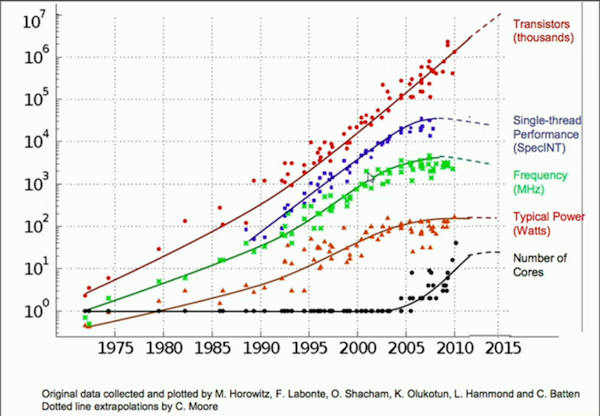
\includegraphics[scale=0.7]{images/c02/moore_and_speed.png}
\end{center}

% texto que aparece al pie de la figura
\caption[Ley de Moore]{La ley de Moore\footnotemark{} se ha cumplido de forma empírica tal como indica la ilustración durante los últimos 40 años. En particular, se evidencia cómo han aumentado la cantidad de transistores en los procesadores. Al mismo tiempo, se observa la tendencia de incrementar el número de núcleos durante los últimos años, sosteniendo la afirmación de que ante la incapacidad de mantener un aumento en la frecuencia del reloj, se ha optado por cambiar las arquitecturas de los procesadores modernos dando paso a esquemas de paralelismo.}
\label{c02_moore_law} % etiqueta para ser usada por referencias desde el texto
\end{figure}
\footnotetext{Fuente: \url{https://www.karlrupp.net/2015/06/40-years-of-microprocessor-trend-data/}}

En los últimos años, se ha experimentado un estancamiento del parámetro de la velocidad del reloj \cite{ross2008cpu}, lo que ha impulsado el desarrollo de arquitecturas más eficientes. Uno de los enfoques por los que se ha inclinado el mercado ha sido el paralelismo. En lugar de tener solo una unidad de cómputo, es que se ha optado por aumentar la cantidad de núcleos distribuyendo así la carga de trabajo en diferentes unidades de cálculo permitiendo de esta manera aumentar el \textit{multi-tasking} y diseñar sistemas energéticamente más eficientes. El paralelismo ha impulsado la necesidad de desarrollar técnicas donde el trabajo realizado por el procesador sea computado por más de un núcleo. Para afrontar el desafío anterior, se debe por un lado, tener una arquitectura de hardware que permita más de un núcleo computacional con la comunicación respectiva entre estos y por otro lado, se debe enfrentar el problema a nivel de software, dividiendo el problema original en tareas más pequeñas para posteriormente reunir las sub-soluciones de cada una de las tareas en la solución general del problema inicial. Es importante mencionar, que no todos los problemas son paralelizables y por lo anterior, no ven un beneficio en dicha arquitectura. Es esperable que en una aplicación computacional se puedan encontrar secciones de código paralelizables y otras que solo pueden implementarse de manera secuencial. Esto resulta que la ganancia máxima que puede otorgar el paralelismo está limitada por lo que se conoce como la Ley de Amdalh \cite{Amdahl:1967:VSP:1465482.1465560}.

\subsubsection{Límites del paralelismo}

Existen dos leyes fundamentales en la computación distribuida las cuales rigen los límites teóricos de ganancia que puede obtener una aplicación al paralelizarse. En primer lugar se encuentra la Ley de Amdalh la cual se define según la fórmula \ref{amdalh_formula}.

\begin{equation}
\label{amdalh_formula}
    S_{latency}\left ( s \right ) = \frac{1}{\left ( 1-p \right ) + \frac{p}{s}}
\end{equation}

Donde:
\begin{itemize}
    \item $S_{latency}$ representa la mejora teórica de la ejecución del programa
    \item $S$ es el beneficio en la sección paralelizable
    \item $P$ es la porción de la ejecución que ve beneficio en el paralelismo
\end{itemize}

Deducible por la misma fórmula es que aún cuando la sección paralelizable vea grandes beneficios, el rendimiento de la ejecución total de la aplicación estará siempre limitada por la sección que no ve beneficio en el paralelismo.
\\
\\
Posteriormente, John L. Gustafson formuló la ley de Gustafson \cite{Gustafson:1988:RAL:42411.42415} donde realizó ciertas revisiones a la ley de Amdalh proponiendo en cambio que la carga de trabajo de la ejecución cambia en la medida que mejoran los recursos disponibles. De esta manera, en la medida que los equipos mejoran, los problemas más grandes se pueden resolver en el mismo tiempo. La formula \ref{gustafson_formula} resume su análisis.

\begin{equation}
\label{gustafson_formula}
    S_{latency}\left ( s \right ) = 1 - p + sp
\end{equation}

Debido al enfoque que toma Gustafson al formular su ley, se puede decir que este es más optimista en cuanto a los beneficios del paralelismo que la ley de Amdalh.





    % Objetivos

\chapter{Titulo 3}
\label{c3} % la etiqueta para referencias




    % Metodología

\chapter{Titulo 4}
\label{c4} % la etiqueta para referencias
    % Prototipo

\chapter{Resultados}
\label{c5} % la etiqueta para referencias


Mostrar, analizar y discutir los principales resultados.     % Resultados

\chapter{Conclusiones}
\label{c6} % la etiqueta para referencias

Las conclusiones hacen lo siguiente:

\begin{itemize}
    \item Primero re-enuncian lo que se hizo, brevemente.
    \item Reflejando los objetivos generales y especificos, se comenta como se cumplieron esto.
    \item Se reflexiona sobre lecciones generales aprendidas, como son distintos de otros resultados, etc.
    \item Entregan futuras direcciones de trabajo, opcionalmente, dependiendo de si hay lineas muy claras para seguir. 
\end{itemize}    % Conclusiones y Trabajo Futuro

% Ingenieros prefieren la bibliografia antes que los anexos

\cleardoublepage

\addcontentsline{toc}{chapter}{Bibliografía}

\bibliographystyle{styles/newapa}
\bibliography{buc}

\appendix % seguido de archivos de apendices

\cleardoublepage

% Escribe 'Anexos' en el Indice General
\addcontentsline{toc}{chapter}{Anexos}

\chapter{Glosario}
\label{glossary}

\begin{itemize}
    \item \textbf{API}: API es una sigla que procede de la lengua inglesa y que alude a la expresión \textit{Application Programming Interface} (cuya traducción es Interfaz de Programación de Aplicaciones). El concepto hace referencia a los procesos, las funciones y los métodos que brinda una determinada biblioteca de programación a modo de capa de abstracción para que sea empleada por otro programa informático.
    \item \textbf{Core}: Hace referencia al núcleo computacional, el cual es un procesador individual al interior de la CPU.
    \item \textbf{Cluster}: El término clúster (del inglés \textit{cluster}, que significa grupo o racimo) se aplica a los conjuntos o conglomerados de ordenadores unidos entre sí normalmente por una red de alta velocidad y que se comportan como si fuesen una única computadora.
    \item \textbf{CPU}: La unidad central de procesamiento o unidad de procesamiento central (conocida por las siglas CPU, del inglés: \textit{central processing unit}), es el hardware dentro de un ordenador u otros dispositivos programables, que interpreta las instrucciones de un programa informático mediante la realización de las operaciones básicas aritméticas, lógicas y de entrada/salida del sistema.
    \item \textbf{DLB}: DLB son las siglas de Dynamic Load Balancing, el cual es el nombre que recibe la implementación del rebalanceo dinámico en esta memoria.
    \item \textbf{Framework}: En el desarrollo de software, un framework es una estructura conceptual y tecnológica de soporte definida, normalmente con artefactos o módulos de software concretos, en base a la cual otro proyecto de software  puede ser organizado y desarrollado. Típicamente, puede incluir soporte de programas, bibliotecas y un lenguaje interpretado  entre otros programas para ayudar a desarrollar y unir los diferentes componentes de un proyecto.
    \item \textbf{HPC}: La computación de alto rendimiento (\textit{High performance Computing} o HPC en inglés) es la agregación de potencia de cálculo para resolver problemas complejos en ciencia, ingeniería o gestión. Para lograr este objetivo, la computación de alto rendimiento se apoya en tecnologías computacionales como los clusters, los supercomputadores o la computación paralela. La mayoría de las ideas actuales de la computación distribuida se han basado en la computación de alto rendimiento.
    \item \textbf{Idleness}: Se dice que la CPU esta en estado \textit{idle} cuando no esta siendo utilizado por ningún programa. En este trabajo, se habla de idleness cuando la aplicación en un instante de tiempo dado esta esperando a los otros procesos y no esta utilizando sus recursos para contribuir al desarrollo de la simulación.
    \item \textbf{Infiniband}: InfiniBand es un bus de comunicaciones serie de alta velocidad, baja latencia y de baja sobrecarga de CPU, diseñado tanto para conexiones internas como externas. Sus especificaciones son desarrolladas y mantenidas por la Infiniband Trade Association (IBTA).
    \item \textbf{Malla}: Las mallas representan una aproximación a un dominio geométrico. Esta representará el grado de aproximación que se quiere lograr entre el modelo computacional y la realidad.
    \item \textbf{MPI}: MPI (\textit{Message Passing Interface}, Interfaz de Paso de Mensajes) es un estándar que define la sintaxis y la semántica de las funciones contenidas en una biblioteca de paso de mensajes diseñada para ser usada en programas que exploten la existencia de múltiples procesadores.
    \item \textbf{Nodo}: En esta memoria, la referencia a Nodo, hace alusión a un ordenador individual dentro de un clúster de cómputo.
    \item \textbf{Rank}: MPI permite crear grupos lógicos de procesos al interior de la aplicación donde en cada grupo, los procesos se distinguen entre ellos por medio de un identificador llamado rank. El rank siempre es relativo a un grupo.
    \item \textbf{SHM}: SHM son las siglas de Shared Memory, el cual es el nombre que este trabajo le dio a la creación de canales con \textit{buffers} de memoria compartida para la comunicación.
    \item \textbf{TLP}: TLP son las siglas de Two Level Partitioning, el cual es el nombre que este trabajo le dio a el particionamiento en dos niveles, que considera la información de la topología del cluster para el primer particionamiento y la cantidad de núcleos de cada nodo para el segundo particionamiento.
    \item \textbf{Topología}: En este trabajo, la topología representa el estudio de la geometría del conjunto de ordenadores comunicados entre sí para el intercambio de información, donde cada uno se denomina nodo. Además internamente, cada nodo tiene su topología, donde la información que se rescata de estos es la cantidad de núcleos computacionales que este posee.
\end{itemize}
%\chapter{Resultados}

\section{Coarse}



\chapter{Cluster Uandes}
\label{uandes_cluster}

Parte del inicial desarrollo de la presente memoria consistió en construir junto a un equipo de trabajo de la Universidad De los Andes un cluster de super-cómputo nocturno dentro de la casa de estudios. Dicho cluster fue elaborado con el objetivo de utilizar los recursos de la universidad y experimentar con las diferentes técnicas propuestas la existencia o no de una mejora frente a dichos esquemas de particionamiento. Para el desarrollo del super-computador, se utilizaron 30 de los ordenadores con los que la universidad cuenta en el laboratorio de \textbf{FICA}. El equipo de trabajo espera integrar más nodos en el futuro.

\begin{figure}[H]
\begin{center}
   \includegraphics[scale=0.083]{images/c03/Supercomputador2.JPG}
\end{center}

%texto que aparece al pie de la figura
\caption[Equipo de trabajo Cluster Uandes]{Equipo de trabajo Cluster Uandes (Universidad de los Andes)\footnotemark{}. El equipo elaboró planificó y elaboro el cluster el primer semestre de 2018 y espera terminar las configuraciones finales en septiembre de 2018.}
\label{c03_cluster_uandes_team} % etiqueta para ser usada por referencias desde el texto
\end{figure}
\footnotetext{Fuente: \url{http://www.uandes.cl/noticias/ingenieros-uandes-desarrollan-supercomputador-nocturno-en-laboratorio-de-la-facultad.html}}

A diferencia de Leftraru, el cluster Uandes se elaboró con componentes que no están diseñados para HPC. Por un lado, los nodos de cómputo son computadores de escritorio donde el uso esperado es la ejecución de programas para el alumnado de la Universidad. Al mismo tiempo, la red de trabajo es \textit{ethernet} por medio de un switch convencional. Esta red de trabajo es apropiada para el uso cotidiano dentro de la universidad, pero es extremadamente limitada a la hora de ejecutar aplicaciones de HPC tanto por la latencia como por el ancho de banda que puede proveer, siendo incapaz de sostener el uso intensivo que ciertas aplicaciones de HPC como OpenSees requieren. Al igual que Leftraru, el cluster fue configurado para poder correrse bajo diferentes configuraciones y números de núcleos.


\begin{figure}[H]
\begin{center}
   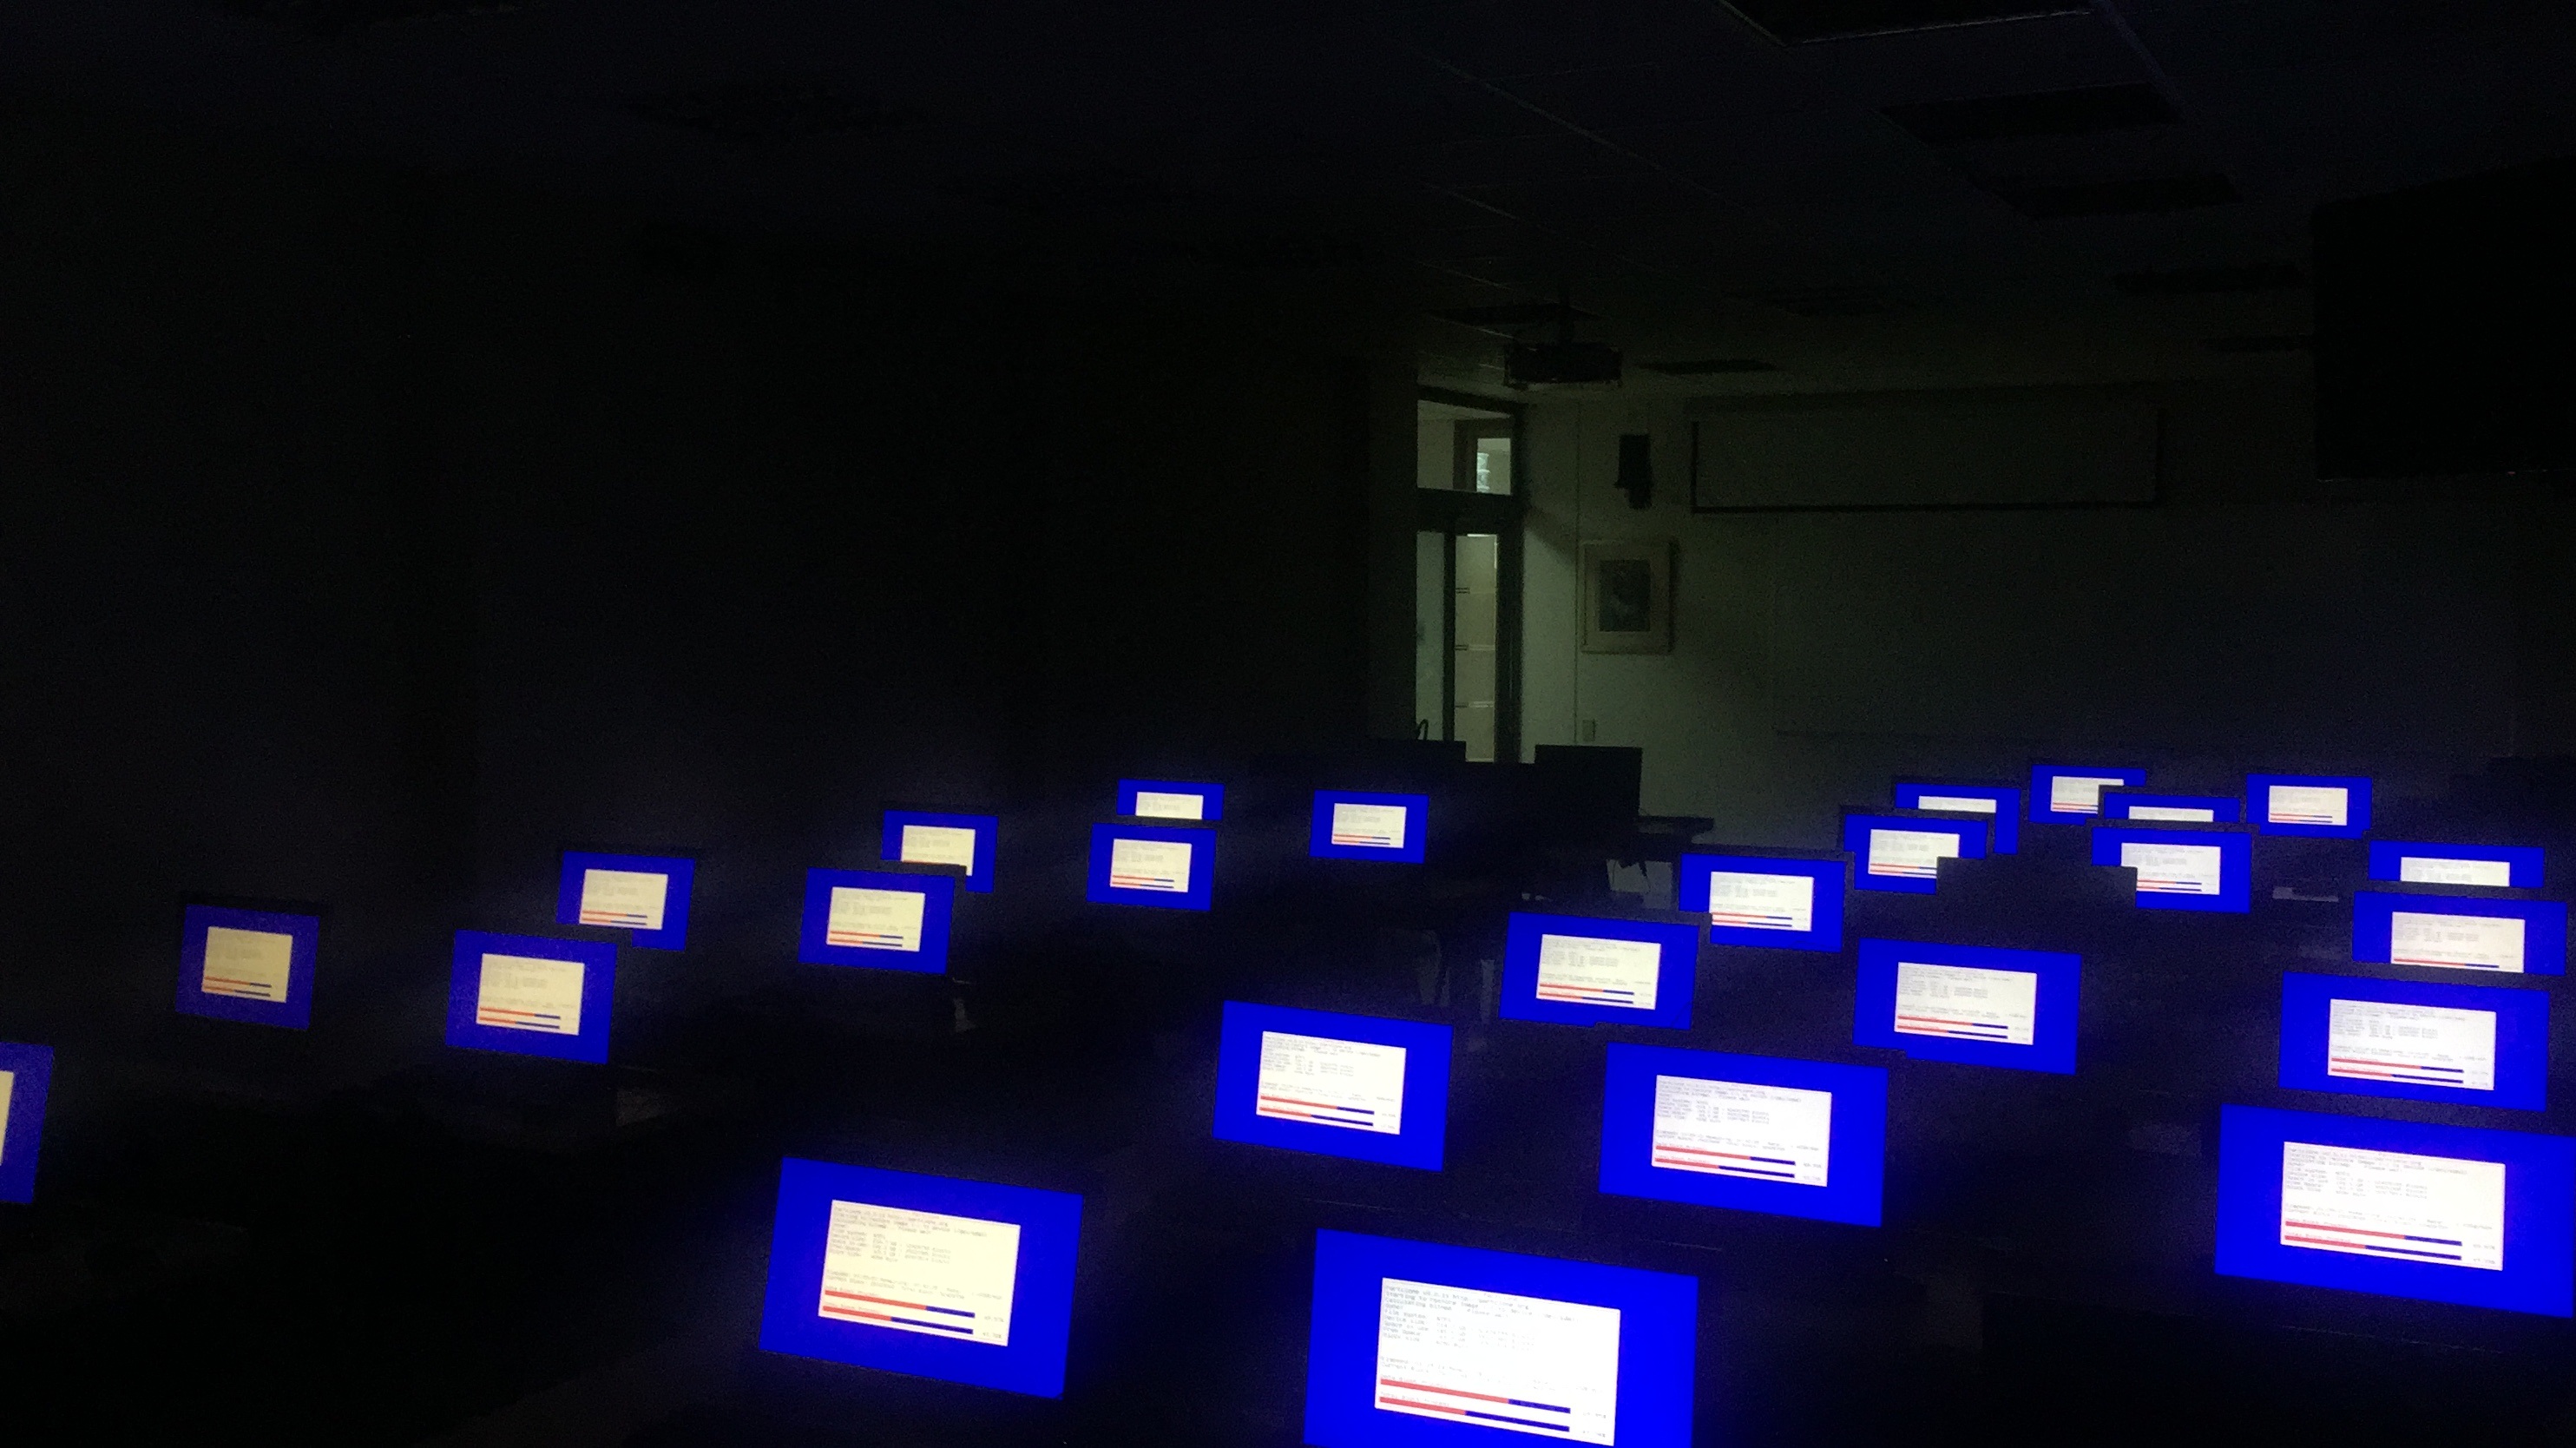
\includegraphics[scale=0.145]{images/c03/cluster_uandes.jpg}
\end{center}

%texto que aparece al pie de la figura
\caption[Cluster Uandes en ejecución]{El Cluster Uandes fue elaborado con el apoyo de la propia Universidad y la facultad de Ingeniería y Ciencias Aplicadas con el objetivo de experimentar con ambientes distribuidos y hacer un uso más efectivo de los recursos de la Casa de estudios. Se pretende que la unidad quede operativa para quedar disponible de manera nocturna frente a las necesidades de los investigadores de la Universidad por medio de una cola de trabajo implementada por Slurm.}
\label{c03_cluster_uandes} % etiqueta para ser usada por referencias desde el texto
\end{figure}

El cluster Uandes posee las especificaciones de la Tabla \ref{table_uandes_cluster_configuration}.

\begin{table}[H]
\begin{tabular}{p{5cm}p{9.3cm}} \toprule
    \textbf{Componente} & \textbf{Descripción}\\ \midrule
    Nombre Cluster & Uandes \\
    Nodos de cómputo & 30 nodos de cómputo Desktop Dell 3050 AIO Series\\
    Cantidad de cores & 120 \\
    Co-Procesadores & No \\
    RAM & 480 GB de RAM \\
    Conexión & Ethernet\\
    Almacenamiento & N/A\\
    Capacidad de cómputo & N/A \\
    \bottomrule

\end{tabular}
\caption[Especificaciones cluster Uandes]{Especificaciones cluster Uandes}
    \label{table_uandes_cluster_configuration}
\end{table}

Se espera que durante el segundo semestre de 2018, las simulaciones ejecutadas en el cluster Leftraru sean replicadas en el super-computador Uandes para determinar así cómo inciden los esquemas de particionamiento en la topología del cluster.


\label{end}
\end{document}

%%%%%%%%%%%%%%%%%%%%%%%%%%%%%%%%%%%%%%%%%%%%%%%%%%%%%%%%%%%%